\def\draft{0}
\documentclass[11pt]{report}
\usepackage{amsfonts, fullpage, rotating, amssymb}
\usepackage{color,amsmath}
\usepackage{IEEEtrantools}
\usepackage{multirow}
\usepackage{hyperref}
\usepackage{amsfonts, fullpage, rotating, amssymb}
\usepackage{color,amsmath}
\usepackage{IEEEtrantools}
\usepackage{multirow}
\usepackage{tcolorbox}
\usepackage{bbm}
\usepackage{hyperref}
\newtheorem{theorem}{Theorem}
\newtheorem{conjecture}{Conjecture}
\newtheorem{definition}{Definition}
\newtheorem{lemma}{Lemma}
\newtheorem{proposition}{Proposition}
\newtheorem{property}{Property}
\newtheorem{corollary}{Corollary}
\newtheorem{claim}{Claim}
\newtheorem{fact}{Fact}
\newtheorem{openprob}[theorem]{Open Problem}
\newtheorem{remk}{Remark}
\newtheorem{exmp}{Example}
\newtheorem{apdxlemma}{Lemma}
\newenvironment{example}{\begin{exmp}
\begin{normalfont}}{\end{normalfont}
\end{exmp}}

\newenvironment{remark}{\begin{remk}
\begin{normalfont}}{\end{normalfont}
\end{remk}}
\newtheorem{sublemma}[theorem]{Sublemma}

\newenvironment{intuition}[1][]{\begin{tcolorbox}[title=Intuition ~(#1),fonttitle=\sffamily\large\bfseries]}{\end{tcolorbox}}

%%%%%%%%%%%%%%%%%%%% proof environments

\def\FullBox{\hbox{\vrule width 8pt height 8pt depth 0pt}}

\def\qed{\ifmmode\qquad\FullBox\else{\unskip\nobreak\hfil
\penalty50\hskip1em\null\nobreak\hfil\FullBox
\parfillskip=0pt\finalhyphendemerits=0\endgraf}\fi}

\def\qedsketch{\ifmmode\Box\else{\unskip\nobreak\hfil
\penalty50\hskip1em\null\nobreak\hfil$\Box$
\parfillskip=0pt\finalhyphendemerits=0\endgraf}\fi}

\newenvironment{proof}{\begin{trivlist} \item {\bf Proof:~~}}
  {\qed\end{trivlist}}
\newenvironment{solve}{\begin{trivlist} \item {\bf Solve:~~}}
  {\qed\end{trivlist}}
\newenvironment{proofsketch}{\begin{trivlist} \item {\bf
Proof Sketch:~~}}
  {\qedsketch\end{trivlist}}

\newenvironment{proofof}[1]{\begin{trivlist} \item {\bf Proof
#1:~~}}
  {\qed\end{trivlist}}

\newenvironment{claimproof}{\begin{quotation} \noindent
{\bf Proof of claim:~~}}{\qedsketch\end{quotation}}


%%%%%%%%%%%%%%%%%%%%%%% text macros
\newcommand{\etal}{{\it et~al.\ }}
\newcommand{\ie} {{\it i.e.,\ }}
\newcommand{\eg} {{\it e.g.,\ }}
\newcommand{\cf}{{\it cf.,\ }}

%%%%%%%%%%%%%%%%%%%%%%% general useful macros
\newcommand{\eqdef}{\mathbin{\stackrel{\rm def}{=}}}
\newcommand{\R}{{\mathbb R}} % real numbers
\newcommand{\N}{{\mathbb{N}}} % natural numbers
\newcommand{\Z}{{\mathbb Z}} % integers
\newcommand{\F}{{\mathbb F}} % a field
\newcommand{\Q}{{\mathbb Q}} % the rationals
\newcommand{\poly}{{\mathrm{poly}}}
\newcommand{\polylog}{{\mathrm{polylog}}}
\newcommand{\loglog}{{\mathop{\mathrm{loglog}}}}
\newcommand{\zo}{\{0,1\}}
\newcommand{\suchthat}{{\;\; : \;\;}}
\newcommand{\pr}[1]{\Pr\left[#1\right]}
\newcommand{\deffont}{\em}
\newcommand{\getsr}{\mathbin{\stackrel{\mbox{\tiny R}}{\gets}}}
\newcommand{\Exp}{\mathop{\mathrm E}\displaylimits} % expectation
\newcommand{\Var}{\mathop{\mathrm Var}\displaylimits} % variance
\newcommand{\xor}{\oplus}
\newcommand{\GF}{\mathrm{GF}}
\newcommand{\eps}{\varepsilon}
\newcommand{\limT}{\lim_{T\rightarrow\infty}}
\newcommand{\limn}{\lim_{n\rightarrow\infty}}
\DeclarePairedDelimiter\ceil{\lceil}{\rceil}
\DeclarePairedDelimiter\floor{\lfloor}{\rfloor}
%%%%%%%%%%%%%%%%%%% macros particular to this course


\pagestyle{plain}
\newcommand{\scribe}{Wei-Chang Lee, Chi-Ning Chou}
\newcommand{\lecnum}{4}
\newcommand{\lecdate}{\today}

%\parskip=1.5mm
%\parindent=0mm
\begin{document}

\tableofcontents

%%%%%%%%%%%%
%	Chapter: 0924    %
%%%%%%%%%%%%
\chapter{0914}
\paragraph{Questions}
\begin{enumerate}
	\item What's the difference between {\bf probability} and {\bf statistics}?
	\item What's the difference between them and {\bf math}?
\end{enumerate}
{\bf Prof. Chaing:}
Mathematics is in a  {\color{red} deterministic}  environment. With math, we can describe a dynamic system in a deterministic way. Probability involves in a probabilistic system, where the events follow certain distribution and act in like flipping a coin. As to statistics, what we face is not beautiful mathematical objects. Instead, we have to deal with {\color{red} data}. We assume there is a distribution or general function behind the data. This function might be deterministic or probabilistic. What a statistician aim to do is to find out (formally speaking, estimate) such underlying distribution.

\section{Probabilities, Random variables, Distribution}
\subsection{Set Theory}
In the world of probability and statistics, we use {\bf set} to intuitively model the object we concerned. As a result, we need to define some basic elements and operations. Furthermore, we will derive some basic properties.
\paragraph{Sample space}
Here we use $\Omega$ to represent sample space, which is composed of all the possible {\bf outcomes}. The element in sample space is often denote as $\omega$.
\paragraph{Event}
What we really care about is the subset of sample space, which is intuitively being an event. With this notion, we can interact with various outcomes and play with events that share the common outcomes etc.
\paragraph{Set operations} Here, we use $A,B,\{A_n\}$ to denote events and a sequence of events.
\begin{itemize}
	\item Union: $A\cup B := \{w:w\in A\ or\ w\in B \}$
	\item Intersection: $A\cap B := \{w:w\in A\ and\ w\in B \}$
	Here, we can drop out the geometric notion of intersection and think of it as {\bf the outcomes that the two events share}.
	\item Complementation: $A^C:=\{w:w\in\Omega\ and\ w\notin A \}$
	The outcomes that haven't happened?
	\item Set difference: $B\backslash A:= B\cap A^C$
\end{itemize}

\paragraph{limsup}
Intuitively, it's analogous to the smallest upper bound for an infinite sequence.
$$\lim\sup A_n := \bigcap_{n=1}^{\infty}\bigcup_{k=n}^{\infty} A_k$$
If we let $B_n:=\bigcup_{k=n}^{\infty} A_k$, we can see that $B_1\supseteq B_2\supseteq...$. Formally, we also have
$$\lim\sup A_n = \{w:w\in A_n, for\ infinitely\ many\ n \}$$
Intuitively, $B_k$ is the outcomes that share by all the events with index greater than $k$.
Or, for any element $\omega$ and barrier $m$, $\exists n\geq m$ such that $\omega\in A_n$.

\paragraph{liminf}
It's the analogy to the largest lower bound for an infinite sequence.
$$\lim\inf A_n:= \bigcup_{n=1}^{\infty}\bigcap_{k=n}^{\infty} A_k$$
If we let $C_n:= \bigcap_{k=n}^{\infty} A_k$, we can see that $C_1\subseteq C_2\subseteq...$. Formally, we also have
$$\lim\inf A_n=\{w:w\in A_n\ for\ all\ but\ finite\ many\ n \}$$
Or, for any element $\omega$ in $\lim\sup A_n$, $\exists m$ such that $\forall n\geq m$, $\omega\in A_n$. That is, after some barrier, $\omega$ will appear in all $A_n$ afterwards.

\paragraph{Limit of sequence of events}
We say a sequence of events $\{A_n\}$ converges to event $A$ if 
$$\limsup A_n=\liminf A_n = A$$

\begin{property}
	Let $A,B,C$ be events in sample space $\Omega$, then the following results hold:
	\begin{enumerate}
		\item Community: $A\cap B=B\cap  A$, $A\cup B=B\cup A$
		\item Associativity: $A\cap(B\cap C) = (A\cap B)\cap C$, $A\cup(B\cup C)=(A\cup B)\cup C$
		\item Distributed law: $A\cap(B\cup C) = (A\cap B)\cup(A\cap C)$, $A\cup(B\cap C)=(A\cup B)\cap(A\cup C)$
		\item De Morgan's law: $(A\cap B)^C = A^C\cup B^C$, $(A\cup B)^C = A^C\cap B^C$
	\end{enumerate}
\end{property}

\section{Small talk}
{\bf Prof. Chiang:} Can you give an example about statistics?\\
{\bf Me:} SVM\\
{\bf Prof. Chiang:} What is SVM?\\
{\bf Me:} blablabla...\\
{\bf Prof. Chiang:} For me, SVM and others techniques are just a chance mechanism. They provides a model or platform for us to analysis the data in some way. But deep in to the heart of data analysis, what we deal with is a general function $G(y,x_1,...,x_k)$. And all techniques are to model the $G$ with certain assumption and structures.

%%%%%%%%%%%%
%	Chapter: 0917    %
%%%%%%%%%%%%
\chapter{0917}
On Monday, we define the idea of set and the operation over it. Intuitively, we think of the element of sets as an {\bf outcome} and think of a set as an {\bf event}. With these notion, further we want to design {\bf chance mechanism} on them to describe real world.

Here comes the important issues:
\begin{itemize}
	\item What kinds of domain (event space) for us to work on?
	\item What kind of chance mechanism (probability function) can we choose?
\end{itemize}
The critical concepts here is that we want to define {\bf axioms} for these two mathematical objects. Moreover, we want such axioms to be
\begin{itemize}
	\item Complete: Close under any possible operations.
	\item Compact: Less number of axioms as possible.
\end{itemize}

\section{Recall}
\subsection{limsup and liminf}
Intuitively, we think of sup and inf as:
\begin{itemize}
	\item sup: Upper bound. In set theory, we think of it as {\bf union} since it contains every future event.
	\item inf: Lower bound. In set theory, we think of it as {\bf intersection} since every future event contains it.
\end{itemize}
As a result, limsup and liminf is analogous to the {\bf asymptotic} upper bound and lower bound for a sequence of sets.

\subsection{Distributive law \& Partition}
\begin{enumerate}
	\item Consider events $A,B$ and sample space $\Omega$,
	$$B\cap\Omega=B\cap(A\cup A^C)=(B\cap A)\cup(B\cap A^C)$$
	As the sets in the union clause are a partition, distributive law tells us that we can divide the event $B$ into two parts. Here we consider a finite partition so you might not get the feeling. But imagine if the partition is infinite...?
	\item Consider,
	$$A\cup B=(A\cup B)\cap\Omega=(A\cup B)\cap(A\cup A^C)=A\cup(B\cap A^C)=A\cup (B\backslash A)$$
	Geometrically, it's like we union another set $B'=(B\backslash A)$ with $A$ where $A$ and $B'$ are {\bf disjoint}. In a special case: $A_1\supseteq A_2\supseteq ...$, it can be think of as a concentric circle
	\begin{figure}[h]
		\centering
		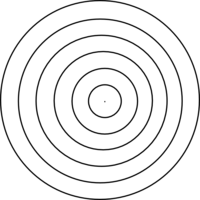
\includegraphics[scale=0.5]{concentric-circle.png}
	\end{figure}
	And thus we can transform an union into a {\bf disjoint union}.
\end{enumerate}

\subsection{General De Morgan's Law}
The De Morgan's law holds true as the number of sets is infinite! Formally, let $\{A_{\alpha}:\alpha\in\Gamma \}$, where $\Gamma$ is an index set and can be infinite, e.g. real line, or time segment. With such notation, we can define something like
$$\bigcup_{\alpha\leq t} A_{\alpha}$$
Which can be the events that happen before time $t$. Then, as De Morgan's law holds true, we can flip the union of events and consider the events that haven't show up. 

Intuitively we can think of this as the {\bf history} or {\bf filtration} in a {\it period sense}. And De Morgan's law provides a convenient way for us to do the computation.

\section{$\sigma$-Algebra}
\subsection{Intuitions and basic axioms}
By definition, $\sigma$-algebra is a collection of subsets of sample space. Intuitively, it is the space of meaningful events. As we mention the {\bf space} of events, $\sigma$-algebra must have some nice properties such as closeness under certain operations etc. But here what we concern is not only about what properties (axioms) a $\sigma$-algebra has to obey, but also about what's the most compact axioms we can have to capture the sufficient and necessary properties a $\sigma$-algebra should follow. And the answer is, there are three of axioms: Consider a $\sigma$-algebra $\mathcal{A}$ over sample space $\Omega$, 
\begin{enumerate}
	\item (contain empty event)$\emptyset\in\mathcal{A}$
	\item (close under complementation)$\forall A\in\mathcal{A}, A^C\in\mathcal{A}$
	\item (close under countable union)$\forall i\in\Gamma\ countable,\ A_i\in\mathcal{A},\ \bigcup_{i\in\Gamma}A_i\in\mathcal{A}$
\end{enumerate}
As a quick remark, we can see that with these axioms, we also have
\begin{itemize}
	\item $\Omega\in\mathcal{A}$ (by 1,2)
	\item Close under countable intersection (by 2, and De Morgan's law)
\end{itemize}

\subsection{Properties}
After defining the basic axioms for all $\sigma$-algebra, now a more applied issue arises:
$$What's\ the\ smallest\ \sigma-algebra?$$
With some observation, we can easily find out the largest and smallest $\sigma$-algebra over sample space $\Omega$ is
\begin{itemize}
	\item Trivial $\sigma$-algebra: $\{\emptyset,\Omega \}$
	\item Total $\sigma$-algebra: $\{A:A\subseteq\Omega \}$. That is, the power set of $\Omega$.
\end{itemize}
To answer this question, we have to clarify some concepts: How do we compare the size of two $\sigma$-algebras and to what extent do we want? The first question can be answered with strictly inclusion. If $\sigma$-algebra $\mathcal{A}_1$ strictly contains $\sigma$-algebra $\mathcal{A}_2$, then we can think of $\mathcal{A}_1$ is larger than $\mathcal{A}_2$. 

As to the second question, we can think this in a reverse way: What elements (subsets of $\Omega$) we must have? This question is problem-dependent, so here we imagine that we put all the events that we care into a set $A$. Then, we got a necessary condition for the $\sigma$-algebra that we desire: any $\sigma$-algebra that can describe the chance mechanism we're going to use must at least contain all the set in $A$.

Intuitively, with the above two concepts, it's reasonable to come to a wild guess for the minimal $\sigma$-algebra:
$$The\ intersection\ of\ all\ \sigma-algebras\ that\ contains\ A.$$
However, there's still one last thing to check: Is the (countable) intersection of $\sigma$-algebras also a $\sigma$-algebra? This can be proved in a theorem.
\begin{theorem}[$\sigma$-algebras are close under countable intersection]
	\mbox{}
	
	If $\mathcal{A}_{\alpha}$ is a $\sigma$-algebra $\forall \alpha\in\Gamma$, where $\Gamma$ is a countable index set. Then $\bigcap_{\alpha\in\Gamma}A_{\gamma}$ is also a $\sigma$-algebra.
\end{theorem}
\begin{proof}
	We should check three things and it's quite trivial. I believe I will never forget so here I leave it blank.
\end{proof}


\section{Probability Function}
Finally, it's time for us to construct the {\bf chance mechanism}! That is, we want to design probability function that maps from a $\sigma$-algebra to $[0,1]$. Moreover, such probability function should be analogous to real life. Namely, not every function from $\sigma$-algebra $\mathcal{A}$ to $[0,1]$ can be out candidate. As a result, we want to design rules (axioms) for probability function in advance. And just as the axioms for $\sigma$-algebra, we hope such axioms can be both compact and complete.

\paragraph{Komolgorov Axioms}
Consider sample space $\Omega$ and a $\sigma$-algebra $\mathcal{A}$ over it. Then, a probability function $P$ should satisfy the following axioms:
\begin{itemize}
	\item (Lower bound) $P(A)\geq0, \forall A\in\mathcal{A}$
	\item (Upper bound) $P(\Omega)=1$
	\item (Countably additive) If $A_{\alpha}\in\mathcal{A},\forall \alpha\in\Gamma$, where $\Gamma$ is a countable {\bf mutually exclusive} index set. Then, $P(\bigcup_{\alpha\in\Gamma}A_{\alpha})=\sum_{\alpha\in\Gamma}P(A_{\alpha})$
\end{itemize}
Note that this brings us from set functions to {\bf value function}. That is, we no longer playing only with set, but also take account the number, i.e. the probability.

Formally speaking, we say $(\Omega,\mathcal{A},P)$ is a probability space if $\mathcal{A}$ is a $\sigma$-algebra over $\Omega$ and $P$ is a probability function.

It's no hard to see that the most important axioms in Komolgorov axioms is countably additive. It allows us to deal with a countably infinite sequence of events. But you must wonder, can we relax the countably additive to finitely additive? If so, do we need to add other constraints? The answer is positive. In fact, we have
$$\mbox{Countably additive} = \mbox{Finitely additive} + \mbox{Axiom of continuity}$$

Here, we state the axiom of continuity without proof (left as exercise)
\paragraph{Axiom of continuity}
If a sequence of events $A_1\supseteq A_2\supseteq...$ and $\lim_{n\rightarrow\infty}A_n=\emptyset$, then $\lim_{n\rightarrow\infty}P(A_n)=0$

After defining the axioms of probability function, now we want to design a probability function for our own usage. However, here comes the problem, how to assign probability function for a given usage? A simple theorem tells us that it's sufficient to define an unique probability function with the known probability assignments on {\bf trivial partition}.
\begin{theorem}
	Let sample space $\Omega=\{w_1,w_2,...\}$, assign probability value to each outcome as $p_1,p_2,...\geq0, \sum_i p_i=1$ respectively. Define the probability function $P$ as
	$$P(A):=\sum_{i:w_i\in A}p_i$$
\end{theorem}
With some verification to the axioms of probability function, we can see that $P$ is an unique probability function over $\Omega$ and the $\sigma$-algebra generated by partition $\{w_1,w_2,...\}$.

Intuitively, once we want to design a probability function for our chance mechanism, it's sufficient to assign probability values over a sufficient partition.

\section{Some random notes}

\subsection{Categorical classification/regression}
Suppose we are analyzing data with label set $\{A,B,C\}$ where these labels have no numerical meaning. What can we do? There's a simple solution called: {\bf dummy variable}

The idea is quite simple. Originally, we have a variable $s\in\{A,B,C\}$. But we cannot use $s$ in any regression or numerical model. Now, let's change a way of thinking. We no longer focus on {\bf which } label does $s$ take. Instead, we consider
\begin{align*}
&\mbox{Is $s$ takes label $A$?}\\
&\mbox{Is $s$ takes label $B$?}\\
&\mbox{Is $s$ takes label $C$?}
\end{align*}

Then, we generate {\bf two} dummy variables to {\bf quantify} the above intuition.
\begin{align*}
&x_1:=\left\{ \,
	\begin{IEEEeqnarraybox}[][c]{l?s}
	1,s=A\\
	0,else
	\end{IEEEeqnarraybox}
	\right.\\
&x_2:=\left\{ \,
\begin{IEEEeqnarraybox}[][c]{l?s}
1,s=B\\
0,else
\end{IEEEeqnarraybox}
\right.
\end{align*}

Now, we have two meaning dummy variables that can be fitted into a numerical model!

\subsection{Boole's inequality}
Boole's inequality, a.k.a union bound, provides a simple but useful tools when dealing with asymptotic issues.
\begin{theorem}[Boole's inequality]
	Consider set of events $\{A_{\alpha}:\alpha\in\Gamma\}$. Then we have
	$$P(\bigcup_{\alpha\in\Gamma}A_{\alpha})\leq\sum_{\alpha\in\Gamma}P(A_{\alpha})$$
\end{theorem}

From Boole's inequality, we can derive Borel Cantelli lemma. And from Borel Cantelli lemma, we can define the concept of almost surely convergence.

%%%%%%%%%%%%
%	Chapter: 0921    %
%%%%%%%%%%%%
\chapter{0921}
Today we're going to talk about some properties of probability function and some useful theorems such as Boole's inequality, Bonferroni's inequality, the first Borel-Cantelli lemma. In the next lecture, we will talk about Counting Theory, and today Prof.Chiang also demonstrate some intuitions about counting theory.

\section{Basic Properties of Probability Function and Their Intuitions}
\begin{theorem}[properties of probability function]
	Suppose $(\Omega,\mathcal{A},P)$ is a probability space where $P$ satisfies the axioms of probability function. Then,
	\begin{enumerate}
		\item (minimizer) $P(\emptyset) = 0$
		\item (finite partition) $P(A) = 1-P(A^C), \forall A\in\mathcal{A}$
		\item (upper bound) $P(A)\leq1, \forall A\in\mathcal{A}$
		\item (conditioned on finite partition) $P(B\backslash A) = P(B\cap A^C) = P(B) - P(B\cap A)$
		\item (union) $P(A\cup B) = P(A) + P(B) - P(A\cup B)$
		\item (sub-event) $P(A)\leq P(B),\forall A,B\in\mathcal{A},A\subseteq B$
		\item (conditioned on countably partition) $P(B) = \sum_{i=1}^{\infty} P(B\cap A_i)$, where $\{A_i\}$ is a partition of $\Omega$ and $A_i\in\mathcal{A},\forall i$.
		\item (Boole's inequality) $P(\bigcup_{i=1}^{\infty}A_i)\leq\sum_{i=1}^{\infty}P(A_i)$. Note that here $\{A_i\}$ is arbitrary sequence of events.
	\end{enumerate}
\end{theorem}

The following gives some intuitions behind each result:
\begin{enumerate}
	\item To prove empty set is a minimizer, we can simply choose a sequence of event as $A_1=\Omega,A_i=\emptyset,\forall i=2,3,...$. Then the results is obvious as we apply countably mutual exclusive additive axiom.
	\item By choosing $A_1=A,A_2=A^C,A_i=\emptyset,\forall i=3,4,...$, countably mutual exclusive additive axiom shows the results.
	\item With 2. and the lower bound axiom.
	\item Consider $B=B\cap\Omega=B\cap(A\cup A^C)$, by distributive law, $B=(B\cap A)\cup(B\cap A^C)$ where the two terms are mutually exclusive. Thus, we an apply the mutually exclusive additive axiom.
	\item By think of $A\cup B$ as $A\cup(B\cap A^C)$ such that the two terms are mutually exclusive. Then consider $B = (B\cap A)\cup(B\cap A^C)$ where the two terms are also mutually exclusive. Apply the mutually exclusive additive axiom, we have $P(A\cup B) = P(A) + P(B\cap A^C) = P(A) + (P(B) - P(B\cap A)) = P(A) + P(B) - P(A\cap B)$.
	\item Simply consider $B=A\cup(B\cap A^C)$.
	\item The same as 4. by consider $B=\bigcup_{i=1}^{\infty} (B\cap A_i)$ where all the terms are mutually exclusive.
	\item Set $A_1^* = A_1, A_2^* = A_2\backslash A_1, A_3^*=A_3\backslash(A_1\cup A_2),...,A_j^*=A_j\backslash(\bigcup_{i=1}^{j-1}A_i)$ such that $\{A_j^*\}$ is mutually exclusive and $\bigcup_{i=1}^{\infty}A_i=\bigcup_{j=1}^{\infty} A_j^*$, which means that $P(\bigcup_{i=1}^{\infty}A_i) = P(\bigcup_{j=1}^{\infty} A_j^*)$. With an observation on $P(A_j^*) = P(A_j\backslash(\bigcup_{i=1}^{j-1}A_i))\leq P(A_j)$, we have $P(\bigcup_{i=1}^{\infty}A_i)\leq\sum_{i=1}^{\infty}P(A_i)$.
\end{enumerate}

\begin{intuition}[properties of probability function]
	The key point here is to make the sets become {\bf mutually exclusive} so that we can apply the mutually exclusive additive axiom. On the contrary, it also shows that the mutually exclusive additive axiom is so strong that what we think is reasonable in intuition can be described by it!
\end{intuition}


\section{Useful Inequalities, and the First Borel-Cantelli Lemma}
In the previous section, Boole's inequality provides an loose upper bound for the probability of the {\bf union} of a sequence of events. Now, we can draw a similar lower bound for the probability of the {\bf intersection} of a sequence of events.
\subsection{Bonferroni's inequality}
\begin{theorem}[Bonferroni's inequality]
	\mbox{}
	
	Let $A_1,A_2,...$ be a sequence of events, then
	$$P(\bigcap_{i=1}^{n} A_i) \geq \sum_{i=1}^{n}P(A_i)-(n-1)$$
\end{theorem}
\begin{proof}
	$$P(\bigcap_{i=1}^{n} A_i) = 1-P(\bigcup_{i=1}^{n}A_i^C) \geq 1-\sum_{i=1}^{n}P(A_i^C) = 1-\sum_{i=1}^{n}(1-P(A_i)) = \sum_{i=1}^{n}P(A_i)-(n-1)$$
\end{proof}

Just as Boole's inequality, Bonferroni's inequality provides a loose lower bound. What does Bonferroni's inequality brings to us? There's an application in {\bf pairwise comparison}: Suppose we are going to estimate three parameters $\theta_1,\theta_2,\theta_3$ which are highly correlated. How can we lower bound the probability of the event: $(\theta_1-\theta_2)\in A_{12},(\theta_1-\theta_3)\in A_{13},(\theta_2-\theta_3)\in A_{23}$? Note that this probability is used for constructing confidence interval.

Now, consider that we have already lower bound the significant level of each parameter, say
\begin{align*}
&P(\theta_1-\theta_2\in A_{12})\geq 1-\alpha_1\\
&P(\theta_1-\theta_3\in A_{13})\geq 1-\alpha_2\\
&P(\theta_2-\theta_3\in A_{23})\geq 1-\alpha_3\\
\end{align*}
By Bonferroni's inequality, we have
\begin{align*}
&P((\theta_1-\theta_2)\in A_{12},(\theta_1-\theta_3)\in A_{13},(\theta_2-\theta_3)\in A_{23})\\
\geq\ &P(\theta_1-\theta_2\in A_{12}) + P(\theta_1-\theta_3\in A_{13}) + P(\theta_2-\theta_3\in A_{23}) - 2\\
\geq\ &(1-\alpha_1) + (1-\alpha_2) + (1-\alpha_3) - 2\\
=\ &1 - (\alpha_1+\alpha_2+\alpha_3)
\end{align*}

\begin{intuition}[Boole's and Bonferroni's inequalities]
	The important concept here is that both Boole's and Bonferroni's inequalities are relatively {\bf loose}. As a result, they can only provide good estimate as the probability of the individual events are {\bf small}. Take a look at the above example, we can see that normally the significant level $\alpha_i$ is relatively small. And that's why here Bonferroni's inequality has some usage.
\end{intuition}

\subsection{The first Borel-Cantelli lemma}
Before we give the statement of the first Borel-Cantelli lemma, let's consider the following motivation:
Imagine after defining the axiom of probability and deduce some nice properties and now you're going to define the concept of {\bf conditional probability} $P(A|B)$. However, an issue coming out:
$$\mbox{What if P(B)=0?}$$
This makes sense as now we consider the sample space with countably many outcomes. The probability of a single outcome is measure 0 ($P(\mbox{outcome}) = 0$). As a result, the conditional probability taught in elementary probability $P(A|B) = \frac{P(A\cap B)}{P(B)}$ is not well-defined!

A simple idea is to relax $B$ or construct a sequence of event $B_1,B_2...$ such that $\lim_{n\rightarrow\infty}B_n = B$ and define the conditional probability as $P(A|B) := \lim_{n\rightarrow\infty}\frac{P(A\cap B_n)}{P(B_n)}$, which is much more making sense. But here comes a question:
$$\mbox{Is the probability of a convergent sequence of events also converge?}$$

\begin{theorem}[The first Borel-Cantelli lemma]
	\mbox{}
	
	Let $\{A_i\}$ be a sequence of events such that $\sum_{i=1}^{\infty}P(A_i)<\infty$, then
	$$P(A_{n.i.o}) = 0$$
	, where $A_{n.i.o} = \limsup_{n\rightarrow\infty}A_n$
\end{theorem}
\begin{proof}
	By the definition of limsup, we have $\bigcup_{i=n}^{\infty} A_i\rightarrow \limsup_{n\rightarrow\infty}A_n$ monotonously. Now, we proof the lemma with two steps:
	\begin{enumerate}
		\item (Continuity axiom) $P(A_{n.i.o}) = \lim_{n\rightarrow \infty}P(\bigcup_{i=n}^{\infty}A_i)$
		\item (Boole's inequality)  $P(\bigcup_{i=n}^{\infty}A_i)\leq\sum_{i=n}^{\infty}P(A_i)$
	\end{enumerate}
	Since $\sum_{i=1}^{\infty}P(A_i)<\infty$, we now that $\lim_{n\rightarrow\infty}\sum_{i=n}^{\infty}P(A_i)=0$. Thus, $P(A_{n.i.o})=0$.
\end{proof}

Note that there's no independence involves here, which is different from the second Borel-Cantelli's lemma that we'll introduce later.

\section{Intuitions About Counting Theory}
$$\mbox{\it Why do we need counting techniques?}$$
\subsection{Sampling}
What kind of sampling mechanisms do we have? That is, how do we design the mechanism for us to draw samples from a large population? Do we sample periodically? Or, sample from the subset that we believe is more important? Or, we cluster the sample space into a smaller subspace and sample in them respectively?

The chance mechanism we choose will affect the underlying possibility for us to get a certain outcome. That is, the way we analyze or the model we choose will differ as the sampling techniques are distinct. And how do we react to different mechanism is to utilize the tools in counting theory.

\subsection{Bootstrap}
In high-dimensional statistics, the number of parameters are so large that sometimes even the number of samples is less than that of parameters! However, we believe the underlying structure might not be so much. Namely, there might exist some sparse or low rank structure behind the scheme.

But, how can we find out such implicit properties with only a few samples and a great amount of candidate parameters? There's a method called {\bf bootstrap}, which reuses the same samples and generate  a subset of new samples from it. With some counting argument, we can see that this will not affect the performance and can increase the number of samples to search for special structure in a high-dimensional setting.

To fulfill such methods, we need to have some tools to analyze the process of reusing samples. And counting theory can provide a great help. For now, this applications give us a sense of motivation to study counting theory.


%%%%%%%%%%%%
%	Chapter: 0924    %
%%%%%%%%%%%%
\chapter{0924}
Today we're going to talk about method of counting to be able to study probability assignments on finite space, we will then give definition about conditional probability on discrete case and intuition about continuous case. After knowing how to calculate conditional probabilities, we can then use Bayes' theorem to connect experimental study to observation study which is called the odds ratio. At the end of the class, Prof.Chiang introduce the concept "independence" and how to interpret it beyond geometric views in a more statistical way.
\section{Counting Methods}
  There are two kinds of interpretation of probability measure. 
\begin{enumerate}
\item[1]
  The first kind of view is based on the "frequency of occurrence". They do random experiments many times to study  how many times event which is interested in would take place. Then, they assign the limit ratio  as the probability of certain events. The intuition of this interpretation is that we believe the underlying parameter is invariant so after many repeated experiment the random effect can be cancelled out and the real instinct reveals. 
\item[2]
  The second kind of view is just based on the "subjective belief of interpreter" in the chance of an event occurring.  We can just give probability under our faith before any experiment has been done and then do experiment to study whether our prior assumption fit the data or not and then modify it. This procedure can be done by Bayes' theorem. 
\end{enumerate}
\paragraph{}
  The counting problem is sometimes sophisticated and along with many restrictions. The way to solve such problem is to break them into series of simple tasks and apply rules to combine it back. 
\begin{theorem}[Fundamental Theorem of Counting]
	Suppose a job consists of k separate tasks, the $i$th of which can be done in $n_i$ ways, then entire job can be done in $\prod_{i=1}^k n_i$ ways.
\end{theorem}
\begin{intuition}[Classification of counting methods]
	The proof of Fundamental Theorem of Counting is quite trivial. Sometimes it is better to think of task as partition criteria such as love or hate, different gender or income level then we just construct a sample space $\Omega=\Omega_1\times\Omega_2...\Omega_k$ which is the cartesian product of k criteria we interested in then we can apply the theorem to calculate there are how many possible outcomes.\\
In reality, we may face situation such as replacement and unordered. Replacement means that $n_i=n_{i+1}$ and unordered means that we can perform k separate tasks arbitrary without certain order. In such case we have to carefully apply or modify the fundamental counting theorem. 	
\end{intuition}
Consider number of possible arrangements of size r drawing from n different subjects. We can divide the case into four categories.
\begin{table}[h]
\centering
\begin{tabular}{lll}
          & Without replacement                                                  & With replacement                \\
Ordered   & $n*(n-1)*(n-2)...(n-r+1)=\frac{n!}{(n-r)!}$     & $n*n*n...n=\prod_{i=1}^r n=n^r$ \\
Unordered & $\frac{\prod_{i=1}^r(n-i+1)}{r!}=\frac{n!}{(n-r)!(r!)}=\binom{n}{r}$ & $\binom{n+r-1}{r}$             
\end{tabular}
\end{table}
\begin{proof}
Case 1 and case 2 is quite simple just applying the Fundamental Theorem of Counting. For case 3, r different objects can be permuted in $r*(r-1)*(r-2)...1=r!$ ways but they represent the same arrangement in unordered situation. So we have case 3 equals case 1 divided by r!. Case 4 is the most difficult, we may simply view it as case 2 divided by r! but it will underestimate the possible arrangements since r objects with some of them are of same kind do not construct r! different permutations. A clever way to solve case 4 is to think of r as numbers of coins and place it arbitrary but all into n different box. A coin in $i$th box means in our ultimate arrangements we have one $i$th objects. Consider a small case as n=3 and r=3. Then the following figure is the realization of picking two $2$th object and one $3$th object. And all possible realization cab be expressed as all possible arrangements of 2 $|$ and 3 $O$ which is $\binom{3-1+3}{3}$. 
$$\underline{\quad}^1 |\underline{OO}^2 |\underline{O}^3$$ So for case 4, the answer is $\binom{n-1+r}{r}$.
\end{proof}
\paragraph{}
The counting techniques are useful when the sample space is finite and every possible outcomes in S are equally likely. The probability of certain event can be calculated by the number of outcomes in that event times the probability of each outcome from the countably addictive axiom.
\begin{theorem}[Enumerating outcomes]
Let $\Omega=\{w_1,w_2...w_n\}$ with $P(\{w_i\})=\frac{1}{n}$ $\forall i$ then $P(A)=\sum_{\{w_i\}\in A}P(\{w_i\})=\sum_{\{w_i\}\in A}\frac{1}{n}=\frac{\sharp(A)}{\sharp(\Omega)}$ $\forall A$.
\end{theorem}
\begin{remark}
This is also the classical definition of probability from Pierre-Simon Laplace.
\end{remark} 
\section{Conditional probability}
In reality, we may need to study something like if she is a girl, what is the probability that she wants to get married. Studying these kinds of probabilities under certain situation or restrictions of sample space needs the definition of conditional probability.
\begin{theorem}
Let P(.) be a probability measure on $\sigma$-algebra $F$, A and B be events in $F$ and P(B)$>$0 then, $P(.|B)$, the conditional probability of A given B is denoted by  
$$P(A|B)=\frac{P(A\cap B)}{P(B)}$$
\end{theorem}
First we need to verify $P(.|B)$ is a probability measure.
\begin{enumerate}
\item[1] $P(A|B)\geq 0$  $\forall A\in F$ : Since $P(B)>0$ and $P(A\cap B)\geq 0$ because P(.) is a probability measure, then the ratio  $\frac{P(A\cap B)}{P(B)}\geq 0$ $\forall A\in F$.
\item[2] $P(\Omega|B)=1$ : $\frac{P(\Omega\cap B)}{P(B)}=\frac{P(B)}{P(B)}=1$.
\item[3] $A_1,A_2...A_n...\in F$, $A_i\cap A_j=\phi$ then $P(\cup_{i=1}^\infty A_i|B)=\sum_{i=1}^{\infty}P(A_i|B)$ : First notice that $A_1\cap B,A_2\cap B...A_n\cap B...$ are all disjoint then $P(\cup_{i=1}^\infty A_i|B)=\frac{P(\cup_{i=1}^\infty A_i\cap B)}{P(B)}=\frac{P(\cup_{i=1}^\infty (A_i\cap B))}{P(B)}=\frac{\sum_{i=1}^{\infty}P(A_i\cap B)}{P(B)}=\sum_{i=1}^{\infty}P(A_i|B)$.
\end{enumerate}
$P(.|B)$ is indeed a probability measure, but what is its statistical meaning?
\begin{example} 
Consider a case that we need to study how accurate our new AIDS test is, then the sample space is partitioned by two criteria. The test result is positive/negative and the subject has AIDS or not. We have  $\Omega:\{(Test,Disease):T\in\{+,-\},D\in\{+,-\}\}=\Omega_T\times\Omega_D$, then
\begin{align*} 
P(D_+|T_+)=\frac{P(D_+\cap T_+)}{P(T_+)}=\frac{P(\{(D_+,T_-),(D_+,T_+)\}\cap\{(D_+,T_+),(D_-,T_+)\})}{P(\{(D_+,T_+),(D_-,T_+)\})}
\end{align*} 
So the conditional probability is actually the study of how sub-sample space $\Omega_T,\Omega_D$ will affect each other on $\Omega$ i.e. what is the relation between each partition criteria, we may not simply think conditional probability in geometric view.   
\end{example}
\begin{intuition}[Conditional Probability]
Generally speaking, $P(B)>0$ cannot always be satisfied since we may be interested in continuous data such as heights and weights. We face division by zero when study problem like given father is 1.75 tall what is the probability the son is 1.80 tall. We have $P(\text{father is 1.75})=0$ and above definition does not work any more. A natural way to save it is to think of B as a small neighbourhood $(B-\frac{\bigtriangleup}{2},B+\frac{\bigtriangleup}{2})$ so we have $$P(A|B)=\frac{\lim_{\bigtriangleup\rightarrow 0} P(A\cap (B-\frac{\bigtriangleup}{2},B+\frac{\bigtriangleup}{2}) )/\bigtriangleup}{\lim_{\bigtriangleup\rightarrow 0}P(B-\frac{\bigtriangleup}{2},B+\frac{\bigtriangleup}{2})/\bigtriangleup}$$  
Noting that both the numerator and denominator are of change rate form so $P(A|B)$ can be thought of as the intensity of the ratio of change rate.\\
In the previous test-disease example, we can not do medical behavior  relying on uncertified test for moral issue. We may only do the reverse direction test. Do the test to patients who have the disease and what is the test result respond to it. So we have only $P(T_+|D_+)$ and also the prevalence rate of the disease $P(D_+)$. How can we know  $P(D_+|T_+)$? This is where we need the Bayes' theorem.  
\end{intuition}
\begin{example}[Casella 1.3.4]
Three prisoners A,B and C are on death row. The governor decides to pardon one of the three prisoners randomly. He informs the warden of his choice but ask warden to keep it secret. A tries to get the warden to tell him who had been pardoned. The warden refuses so A asks another way. A asks which of B and C will be executed. And the following table is warden's possible react.  
\end{example} 
\begin{table}[h]
\centering
\begin{tabular}{lll}
Pardoned & Warden tells & Probability \\ \hline
A        & B dies       & r           \\
         & C dies       & 1-r         \\\hline
B        & C dies       & 1           \\\hline
C        & B dies       & 1          
\end{tabular}
\end{table}
The warden tells A that B would be executed, does it reveal any message to A?
\begin{solve}
Let W denote the event that warden says B will die then A can update his probability given W.
\begin{align*}
P(\text{A pardoned }|W)&=\frac{P(A\cap W)}{P(W)}\\
&=\frac{P(\text{A pardoned B dies})}{P(\text{A pardoned B dies})+P(\text{C pardoned B dies})+P(\text{B pardoned B dies})}\\
&=\frac{\frac{1}{3}\cdot r}{\frac{1}{3}\cdot r+\frac{1}{3}+0}=\frac{r}{r+1}
\end{align*}
The answer would rely on warden's behavioral pattern.
\begin{table}[h]
\centering
\begin{tabular}{l|ll}
\hline
                & $P(A|W)$      & Message   \\ \hline
$r=1$           & $\frac{1}{2}$ & good news \\ 
$r=\frac{1}{2}$ & $\frac{1}{3}$ & no news   \\ 
$r=0$           & $0$           & bad news  \\ 
\end{tabular}
\end{table}
\begin{intuition}[Three Prisoners]
When r tends to 1, the probability A would be pardoned reaches $\frac{1}{2}$. This is because when A had been pardoned, the warden would always say B and event W becomes a more good predictor of A pandered and vice versa. When $r=\frac{1}{2}$, the warden has the same chance to tell B or C dies when A had been pardoned so W can not be used to trace back A pardoned. Sometimes people may think $P(A|W)=\frac{1}{2}$ because one of A and C would be saved. But it is $P(A|B^C)$ actually. \\
Consider $P(C|W)$ it is actually $1-P(A|W)$. So when $r=\frac{1}{2}$, $P(C|W)=\frac{2}{3}$. Though warden reveals no message to A but it is actually a good news for C. It is like the situation we switch door in the Monty Hall problem. Conditional probability can be really tricky.
\end{intuition}
\end{solve}


\section{Bayes Rule}
\subsection{Bayes rule}
Imagine a situation that there are two sample spaces $\Omega_1 = \{D_1,...,D_p\},\Omega_2 = \{O_1,...,O_q\}$ that augments a larger sample space $\Omega=\Omega_1\times\Omega_2$. What kind of inferences can we draw from the knowledge of outcome $O$? If I know the conditional probability $P(O|D)$ what can do to inference $P(D|O)$?

Intuitively, there are four categories of probabilities here:
\begin{itemize}
	\item $P(D)$: probability of getting disease.
	\item $P(O)$: probability of yielding some symptoms (outcomes).
	\item $P(D|O)$: probability of getting disease conditioned on having some symptoms.
	\item $P(O|D)$: probability of having some symptoms conditioned on getting a disease.
\end{itemize}
The four categories are connected together with the following Bayes rule:
$$P(D = d|O = o) = \frac{P(O=o|D=d)}{\sum_{d\in D}P(D=d)P(O=o|D=d)}$$
The important philosophy here is that, in real life, we won't have all the four categories of probability in hand. That is, we have to draw inference on the probability we care from the probability we known. For example, a doctor want to know the probability of a patient getting disease $d$ conditioned on he has symptom $o$. If the doctor knows the probability of getting a disease ($P(D)$), and the probability of a outcome to happen conditioned on having disease or not ($P(O|D)$). Then, by applying Bayes rule, he can calculate the conditioned probability $P(D|O)$, which is what he concerns.

Here I a little abuse the notation of $D$, actually, the event in $D$ must be a {\bf partition}. For example $D=\{\mbox{disease},\mbox{no disease}\}$.

Now, we formally state the Bayes rule as follow:
\begin{theorem}[Bayes rule]
	Let $A_1,...,A_n$ be a partition over $\mathcal{A}$ and $B\in\mathcal{A}$, then
	$$P(A_i|B) = \frac{P(B|A_i)}{\sum_j P(A_j)P(B|A_j)}$$
\end{theorem}

\begin{intuition}[Bayes rule]
	Bayes rule help us update the probability over a {\bf partition} on event space. It utilize what we have:
	\begin{itemize}
		\item The probability of population on the partition.
		\item The conditioned probability of the observed event conditioned on each event in the partition. 
	\end{itemize}
	Then calculate the conditioned probability we want to inference: The probability of each event in the partition to happen conditioned on an observation.
\end{intuition}

\subsection{Relative risk and Odd ratio}
Both relative risk and odd ratio are important statistical concept in epidemiology/experimental study. In this context, we care the following scenario: There's a disease and a treatment, we want to know how well the treatment is but in the meantime hoping the treatment has less side-effect. We can summarize the above scenario in Table~\ref{table:epidemiology}. Here, $D$ refers to the event that the patient has the disease and $E$ is the event that the patient is under treatment (or formally, being exposed to the treatment). In the context of experimental study, see Table~\ref{table:experimentalstudy}, $E$ can be regarded as the experimental group and $E^C$ can be seen as the control group. Here $D$ and $D^C$ can be simply considered as the presence and absence of an event.

\begin{table}[h]	
	
	\begin{minipage}{.5\textwidth}
		\centering
		\begin{tabular}{|l|l|c|c|}
			\hline
			\multicolumn{2}{|c|}{\multirow{2}{*}{Risk}} & \multicolumn{2}{c|}{Treatment}                                    \\ \cline{3-4} 
			\multicolumn{2}{|c|}{}                      & \multicolumn{1}{l|}{Exposed} & \multicolumn{1}{l|}{Not exposed} \\ \hline
			\multirow{2}{*}{Disease}      & Diseased     & $P(D|E)$                      & $P(D|E^C)$                        \\ \cline{2-4} 
			& Healthy      & $P(D^C|E)$                    & $P(D^C|E^C)$                      \\ \hline
		\end{tabular}
		\caption{Epodemiology scenario.}
		\label{table:epidemiology}
	\end{minipage}
	\begin{minipage}{.5\textwidth}
		\centering
		\begin{tabular}{|l|l|c|c|}
			\hline
			\multicolumn{2}{|c|}{\multirow{2}{*}{Risk}} & \multicolumn{2}{c|}{Experiment}                                    \\ \cline{3-4} 
			\multicolumn{2}{|c|}{}                      & \multicolumn{1}{l|}{Experiment} & \multicolumn{1}{l|}{Control} \\ \hline
			\multirow{2}{*}{Outcome}      & Presence     & $P(D|E)$                      & $P(D|E^C)$                        \\ \cline{2-4} 
			& Absence      & $P(D^C|E)$                    & $P(D^C|E^C)$                      \\ \hline
		\end{tabular}
		\caption{Experimental study.}
		\label{table:experimentalstudy}
	\end{minipage}
\end{table}


With this scenario, we an immediately some intuitive term to help us making inference. The first one is {\bf relative risk (RR)}. Relative risk is the probability ratio of an event to happen under certain exposure or not. In this context, it's simply $\frac{P(D|E)}{P(D|E^C)}$. 
\begin{definition}[relative risk]
	Relative risk (RR) is the probability ratio of an event to happen under an exposure or not. That is
	$$\mbox{RR}:=\frac{P_{event\ when\ exposed}}{P_{event\ when\ not\ exposed}}$$
\end{definition}
Note that RR can help us inference on the effectiveness of the treatment on the disease. See Table~\ref{table:relativerisk} for more details on RR.

\begin{table}[h]
	\centering
	\begin{tabular}{|l|l|l|}
		\hline
		& \multicolumn{1}{c|}{Epidemiology}               & \multicolumn{1}{c|}{Experimental study}                                                     \\ \hline
		RR$>$1 & \parbox{6.5cm}{Thetreatment is worse than having no treatment.} & \parbox{6.5cm}{The event is more likely to happen in the {\bf experimental} group.} \\ \hline
		RR$<$1 & The treatment is effective.                     & \parbox{6cm}{The event is more likely to happen in the {\bf control} group}       \\ \hline
	\end{tabular}
	\caption{Relative risk.}
	\label{table:relativerisk}
\end{table}

Now, we can use relative risk to describe the effectiveness of a treatment/experiment on a certain disease/event, we might wander: how about the relation between two diseases/events under the same treatment/experiment? And this is actually the definition of odd ratio.
\begin{definition}[odd ratio]
	The odd ratio (OD) is the ratio of the relative risk of two events. That is, the odd ratio of event $A$ and $B$ w.r.t a treatment $E$ is
	\begin{align*}
	OD:&=\frac{RR_A}{RR_B}\\
	&=\frac{P(A|E)/P(A|E^C)}{P(B|E)/P(B|E^C)}
	\end{align*}
\end{definition}
The simplest odd ratio is to consider a event and its complement, say $D$ and $D^C$, then the odd ratio will become 
\begin{align*}
\frac{P(D|E)/P(D|E^C)}{P(D^C|E)/P(D^C|E^C)} &= \frac{P(D\cap E)/P(D\cap E^C)}{P(D^C\cap E)/P(D^C\cap E^C)}\\
&=\frac{P(D\cap E)/P(D^C\cap E^C)}{P(D^C\cap E)/P(D\cap E^C)}
\end{align*}

With this transformation, we can use the four intersection probability to calculate the odd ratio instead of the four conditional probability. In some circumstances, this will be more convenient and intuitive.

\section{Independence}
The initial idea (and the most intuitive concept) of independence is that two event $A$ and $B$ is said to be independent if the probability of $A$ to happen will not change after we have the knowledge of $B$, and vice versa. Thus, formally we can write
$$P(A) = P(A|B) = \frac{P(A\cap B)}{P(B)}$$
$$P(B) = P(B|A) = \frac{P(A\cap B)}{P(A)}$$
And we can see that actually as $A$ and $B$ are independent, $P(A\cap B) = P(A)P(B)$, while the converse is also correct. As a result, this has become the definition of independence.
\begin{definition}[independence]
	We say two event $A$ and $B$ are independent if $P(A\cap B) = P(A)P(B)$.
\end{definition}

However, note that there are more than one concept about independence in mathematics. For instance, in linear algebra, there's so called linear independence. And even in probability theory, as we consider more than one event, say a group of events, the idea of independence varies. Actually, there are two kinds of independence for more than two events: {\bf pairwise independence} and {\bf mutually independence}.

\begin{definition}[pairwise independence]
	We say a finite set of events $\{A_i\}$ is pairwise independent if $\forall A_i\neq A_j$, $P(A_i\cap A_j) = P(A_i)P(A_j)$.
\end{definition}
\begin{definition}[mutually independence]
	We say a finite set of events $\{A_i\}$ is mutually independent if for any subset of $\{A_i\}$, say $\{A_j'\}$, $P(\bigcap_{j}A_j')=\prod_{j}P(A_j')$.
\end{definition}

Note that mutually independence is {\bf strictly stronger} than pairwise independence. That is, the former implies the latter while the converse is not necessarily true.

\end{document}




